\input{preamble}
\usepackage{eurosym}
\usetikzlibrary {datavisualization}

\newcommand{\tableaucroise}[4]{
\begin{tabular}{|c|c|c|c|}
	\cline{2-4}
	\multicolumn{1}{c|}{} & #1 \\ \hline
	#2 \\ \hline
	#3  \\ \hline
	#4  \\ \hline
\end{tabular}
}

\begin{document}

\pagestyle{fancy}
\fancyhead[L]{Terminale STMG}
\fancyhead[C]{\textbf{TD n°6 : probabilités conditionnelles}}
\fancyhead[R]{\today}

\exe{}{
On considère deux évènements $A$ et $B$ et on donne :
\begin{multicols}{2}
\begin{enumerate}[label=(\roman*)]
\item $P_{\widebar{B}}(A) = 0,6$
\item $P_B(A) = 0,5$
\item $P(\widebar{B}) = 0,25$
\end{enumerate}
\end{multicols}
\begin{enumerate}
\item
Compléter l'arbre ci-dessous :
\begin{center}
\begin{tikzpicture}[scale=1]
\node {}[grow=right, level distance=4cm, sibling distance=2cm]
	child {node {\small $\widebar{B}$}[level distance=4cm, sibling distance=1cm]
		child {node{\small $\widebar{A}$}			
		}
		child {node{\small $A$}
		}
	}
	child {node {\small $B$}[level distance=4cm, sibling distance=1cm]
		child {node{\small $\widebar{A}$}
		}
		child {node{\small $A$}
		}
	}
;
\end{tikzpicture}
\end{center}
\item Donner $P(A \cap B)$.
\item Calculer $P_A(B)$.
\end{enumerate}
}{exe:arbre1}{

}

% inspi Manuel : indice maths Bordas
\exe{}{
On considère deux évènements $A$ et $B$ et on donne :
\begin{multicols}{2}
\begin{enumerate}[label=(\roman*)]
\item $P(B) = 0,4$
\item $P_B(A) = 0,25$
\item $P(\widebar{B}) = 0,6$
\end{enumerate}
\end{multicols}
On note $p = P_{\widebar{B}}(A)$.
\begin{enumerate}
\item
Compléter l'arbre ci-dessous avec les données de l'énoncé.
\begin{center}
\begin{tikzpicture}[scale=1]
\node {}[grow=right, level distance=4cm, sibling distance=2cm]
	child {node {\small $\widebar{B}$}[level distance=4cm, sibling distance=1cm]
		child {node{\small $\widebar{A}$}			
		}
		child {node{\small $A$}
		}
	}
	child {node {\small $B$}[level distance=4cm, sibling distance=1cm]
		child {node{\small $\widebar{A}$}
		}
		child {node{\small $A$}
		}
	}
;
\end{tikzpicture}
\end{center}
\item Justifier que $P(A) = 0,1 + 0,6 p$.
\item On donne $P(A) = 0,4$, en déduire la valeur de $p$.
\item Compléter toutes les branches de l'arbre pondéré.
\end{enumerate}
}{exe:arbre2}{

}

\exe{}{
On donne l'arbre ci-dessous :
\begin{center}
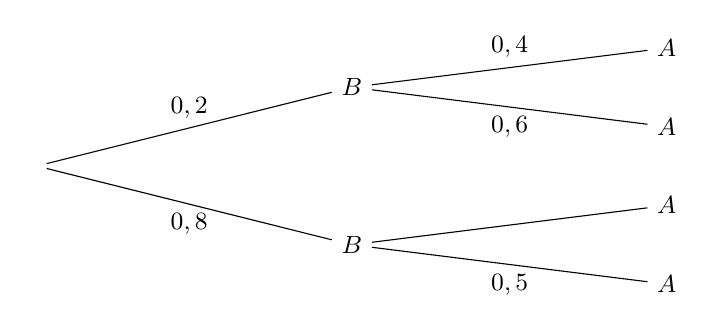
\begin{tikzpicture}[scale=1]
\node {}[grow=right, level distance=4cm, sibling distance=2cm]
	child {node {\small $\widebar{B}$}[level distance=4cm, sibling distance=1cm]
		child {node{\small $\widebar{A}$}
			edge from parent node[below] {\small $0,5$}
		}
		child {node{\small $A$}
			edge from parent
		}
		edge from parent node[below] {\small $0,8$}
	}
	child {node {\small $B$}[level distance=4cm, sibling distance=1cm]
		child {node{\small $\widebar{A}$}
			edge from parent node[below] {\small $0,6$}
		}
		child {node{\small $A$}
			edge from parent node[above] {\small $0,4$}
		}
		edge from parent node[above] {\small $0,2$}
	}
;
\end{tikzpicture}
\end{center}
Donner, ou calculer :
\begin{multicols}{3}
\begin{enumerate}
\item $P(B)$
\item $P(\widebar{B})$
\item $P_B(A)$
\item $P_B(\widebar{A})$
\item $P_{\widebar{B}}(A)$
\item $P_{\widebar{B}}(\widebar{A})$
\item $P(A \cap B)$
\item $P(\widebar{A} \cap B)$
\item $P(A \cap \widebar{B})$
\item $P(\widebar{A} \cap \widebar{B})$
\item $P(A)$
\item $P(\widebar{A})$
\item $P_A(B)$
\item $P_{\widebar{A}}(B)$
\item $P_A(\widebar{B})$
\item $P_{\widebar{A}}(\widebar{B})$
\end{enumerate}
\end{multicols}
}{exe:arbre3}{

}

\exe{}{
Une épidémie de grippe se propage au LJM, on considère :
\begin{enumerate}[label=(\roman*)]
\item que 20 \% des élèves sont infectés ;
\item que si deux élèves sont assis côte à côte lors d'un cours et que si l'un d'eux est infecté, le second a 80 \% de chance d'être contaminé.
\end{enumerate}
Calculer les probabilités suivantes :
\begin{enumerate}
\item La probabilité qu'un élève non contaminé soit infecté après un cours.
\item La probabilité qu'un élève (contaminé ou non) soit infecté après un cours.
\item La probabilité qu'un élève contaminé soit assis à côté d'un élève sain durant un cours.
\item La probabilité qu'un élève infecté contamine un élève sain durant un cours.
\end{enumerate}
\textit{On pourra utiliser des lettres pour désigner les différents évènements}.
}{exe:cond1}{

}

\exe{}{
Une entreprise de location de véhicule a collecté les données suivantes sur sa flotte :
\begin{enumerate}[label=(\roman*)]
\item 30 \% de ses clients louent un véhicule de tourisme (une voiture \og classique \fg) ;
\item 60 \% de ses clients louent un utilitaire ;
\item le reste de ses clients louent des véhicules de sport.
\end{enumerate}
Lors de la restitution des véhicules, l'entreprise estime les dégâts matériels, elle distingue trois catégories :
\begin{enumerate}[label=(\alph*)]
\item pas de dégât matériel ;
\item dégâts matériels légers = préjudice inférieur à 300 \euro{};
\item dégâts matériels importants = préjudice supérieur à 300 \euro.
\end{enumerate}
Enfin, l'entreprise a constaté que :
\begin{enumerate}[label=(\roman*)]
\item 5 \% des véhicules de tourisme loués sont restitués avec des dégâts matériels légers.
\item 1 \% des véhicules de tourismes loués sont restitués avec des dégâts matériels importants.
\item 80 \% des utilitaies loués sont restitués sans dégât matériel ;
\item 5 \% des utilitaires loués sont restitués avec des dégâts matériels importants.
\item 95 \% des véhicules de sport loués sont restitués sans dégât matériel ;
\item 5 \% des véhicules de sport loués sont restitués avec des dégâts matériels importants.
\end{enumerate}
Estimer les probabilités suivantes :
\begin{enumerate}[label=(\alph*)]
\item la probabilité qu'un véhicule loué soit restitué avec des dégâts importants ;
\item la probabilité qu'un client n'ayant pas loué une voiture de sport restitue le véhicule sans dégât matériel ;
\item la probabilité qu'un utilitaire soit restitué avec des dégâts (légérs ou importants) ;
\item la probabilité qu'un client loue un utilitaire et le restitue sans dégât.
\end{enumerate}
}{exe:cond2}{

}

\exe{}{
	On tire une boule dans une urne contenant $2$ boules rouges et $4$ boules vertes.
	\begin{enumerate}[label=(\roman*)]
		\item Si la boule tirée est verte, on la met de côté et on retire une nouvelle boule
		\item Si la boule tirée est rouge, on la remet dans l'urne et on retire une nouvelle boule
	\end{enumerate}
	On distingue les quatre événements suivants :
		\begin{multicols}{2}
		\begin{enumerate}[label=]
			\item v : \og la première boule tirée est verte \fg
			\item r : \og la première boule tirée est rouge \fg
			\item V : \og la deuxième boule tirée est verte \fg
			\item R : \og la deuxième boule tirée est rouge \fg
		\end{enumerate}
		\end{multicols}

	\begin{multicols}{2}
	\begin{enumerate}
		\item Donner $P(\text{v})$ et $P(\text{r})$.
		\item Donner $P(\text{V sachant v})$ et $P(\text{V sachant r})$.
		\item Calculer $P(\text{V $\cap$ v})$ et $P(\text{V $\cap$ r})$.
		\item Calculer $P(\text{V})$ puis $P(\text{R})$.
	\end{enumerate}
	\end{multicols}
}{exe:cond3}{

}

% cf. Manuel : indice maths Bordas
\exe{}{
$A$ et $B$ désignent deux évènements tels que $P(A) = 0,3$ et $P(B) = 0,4$. Calculer $P(A \cap B)$ dans chacun des cas suivants :
\begin{enumerate}[label=(\alph*)]
\item $A$ et $B$ sont indépendants ;
\item $A$ et $B$ sont incompatibles.
\end{enumerate}
\textit{Deux évènements sont dits incompatibles s'ils ne peuvent pas survenir en même temps}.
}{exe:ind1}{

}

\exe{}{
	Une urne contient $49$ billes numérotées de $1$ à $49$.
	La moitié des billes paires sont bleues, les $\frac25$ des billes impaires sont jaunes.
	Compléter le tableau croisé d'effectifs ci-dessous :
	
	\begin{center}
	%\def\arraystretch{1.8}
	\setlength\tabcolsep{20pt}
	\tableaucroise{Paire & Impaire & Total}{Bleue & & &}{Jaune & & &}{Total &&&}
	\end{center}
	
	On choisit une bille uniformément au hasard et on dénote
		\begin{center}
			$I$ : \og La bille a un numéro impair. \fg
			\hspace{3cm}
			$B$ : \og La bille est bleue. \fg
		\end{center}
	Donner $P(I)$ et $P_B(I)$ à l'aide du tableau. Les événements $I$ et $B$ sont-ils indépendants ?
}{exe:ind2}{

}

\exe{}{
On considère $A$ et $B$ deux évènements d'un univers $\Omega$.
\begin{enumerate}
\item Rappeler la formule de probabilité totale appliquée à $P(A)$ (voir cours).
\item En déduire la formule suivante :
\[ P(A) = P(B) \cdot P_B(A) + P(\widebar{B}) \cdot P_{\widebar{B}}(A) . \]
\end{enumerate}
}{exe:probatotale}{

}

% inspi : https://www.bibmath.net/dico/index.php?action=affiche&quoi=./b/bayes.html
\exe{}{
Alors qu'une maladie grave se propage rapidement, un test de dépistage a été mis en place. Ses caractéristiques sont les suivantes :
\begin{enumerate}[label=(\roman*)]
\item si une personne \textbf{est} malade alors le test est positif (détecte la maladie) avec une probabilité de 99 \% ;
\item si une personne \textbf{n'est pas} malade alors le test est positif avec une probabilité de 0,1 \% (on parle de \og faux positif \fg).
\end{enumerate}
On note $M$ l'évènement \og la personne est malade \fg{} et $T$ l'évènement \og le test est positif \fg. 
On suppose qu'une personne sur 10~000 a déjà contracté la maladie.
\begin{enumerate}
\item Donner les valeur de $P(M)$ et $P(\widebar{M})$.
\item Donner la valeur de $P_M(T)$ et $P_{\widebar{M}}(T)$.
\item En utilisant le résultat de l'exercice $\ref{exe:probatotale}$, montrer que :
\[ P(T) = P(M) \cdot P_M(T) + P(\widebar{M}) \cdot P_{\widebar{M}}(T) . \]
\item En utilisant la formule de Bayes, estimer la probabilité qu'une personne soit malade \textbf{sachant} que le test est positif.
\item Conclure sur l'efficacité du test.
\end{enumerate}
}{exe:bayes1}{

}

% inspi Manuel : indice maths Bordas
\exe{}{
Un habitant d'une grande métropole se déplace uniquement en vélo ou en transports en commun.
Si la journée est ensoleillée, alors cette habitant se déplace en vélo 9 fois sur 10.
Sinon, il ne se déplace en vélo que 6 fois sur 10.
On note $p$ la probabilité que la journée soit ensoleillée ainsi que $E$ et $V$ les évènements : 
\begin{enumerate}[label=(\roman*)]
\item E : \og la journée est ensoleillée \fg{};
\item V : \og l'habitant se déplace en vélo \fg.
\end{enumerate}
\begin{enumerate} 
\item Construire l'arbre pondéré représentant cette situation.
\item Montrer que $P(V) = 0,3p + 0,6$.
\item On consate que dans 67,5 \% des cas, l'habitant se déplace en vélo.
\begin{enumerate}
\item Calculer la valeur de $p$.
\item Sachant que l'habitant s'est déplacé en vélo, montrer que la probabilité que la jourée soit ensoleillée est égale à $\dfrac13$.
\end{enumerate}
\end{enumerate}
}{exe:pb1}{

}

%%%%%%%%%%%%%%%%%%%%%%%%%%%%%
%
%\newpage
%\fancyhead[C]{\textbf{Solutions - TD5}}
%\shipoutAnswer

\end{document}